\documentclass[aspectratio=169]{beamer}
\usepackage[utf8]{inputenc}
\usepackage[T1]{fontenc}
\usepackage{tikz}
\usepackage{hyperref}
\usepackage{pgfplots}
\usepackage{pgf-pie}
\usepackage{pgfpages}

\pgfplotsset{compat=1.17}
\usetikzlibrary{patterns}
\setbeameroption{show notes on second screen}
% \pgfpagesuselayout{2 on 1}[a4paper,border shrink=10mm]

\usetheme[darkmode, nofooterlogo]{pureminimalistic}
% \renewcommand{\pageword}{}
\renewcommand{\logotitle}{}
\renewcommand{\logoheader}{}
\renewcommand{\logofooter}{}
\usepackage[backend=biber, doi=false, maxbibnames=2, maxcitenames=2, style=numeric, sorting=none, url=false, eprint=false]{biblatex}
\addbibresource{bibliography.bib}
\usepackage{appendixnumberbeamer}
\renewcommand{\appendixname}{\texorpdfstring{\translate{appendix}}{appendix}}

\title[Debugging of RxJS-based Applications]{The State of Debugging for RxJS\\``Debugging of RxJS-Based Applications''}
\author{Manuel Alabor and Markus Stolze}
\institute{OST in Rapperswil, Switzerland}
\date{\today}

\begin{document}

\maketitle

\note[itemize] {
    \item Welcome
    \item I am Manuel
    \item Frontend Engineer for 7 years
    \item Web and native mobile
    \item Now: Senior Frontend Engineer, Swiss Fintech
    \item Now: Master Student, OST, Switzerland
    \item In my talk about: State of debugging for RxJS
    \item I want to tell a story
}

\section{Introduction}

\subsection{Why?}

\begin{frame}[fragile]{Reactive Programming for the Web}
    \begin{figure}
        \centering
        
\includegraphics[height=0.6\textheight]{figures/frontend-engineers.jpg}
        \label{fig:rxjs}
    \end{figure}
\end{frame}

\note[itemize] {
    \item JS, frontend, frontend engineer...
    \item Are ``Frontend Engineers'' Engineers?
    \item Because of things like RxJS...
    \item Frontend Engineering came a long way!
    \item RxJS is RP with JavaScript
    \item Nice: TypeScript Interface
    \item Nice: RxJS is core part of Googles Angular
    \item Nice: Describe data flows
    \item Wait? Sales pitch?
    \item I have another story:
    \item About: Debugging
}

\begin{frame}[fragile]{Debugging: First Intuition}
    \begin{figure}[H]
        \centering
        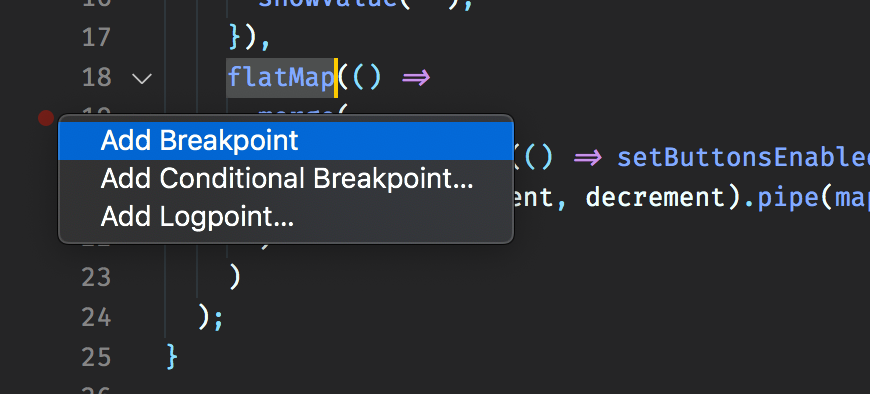
\includegraphics[height=\textheight/2]{figures/add-breakpoint.png}
        \caption{Add a Breakpoint}
    \end{figure}
\end{frame}

\note[itemize] {
    \item Back when i started with RP
    \item Debug? Ha! Breakpoint!
    \item Helped sometimes (lambda functions, ...)
}

\begin{frame}[fragile]{Debugging: First Intuition}
    \begin{figure}[H]
        \centering
        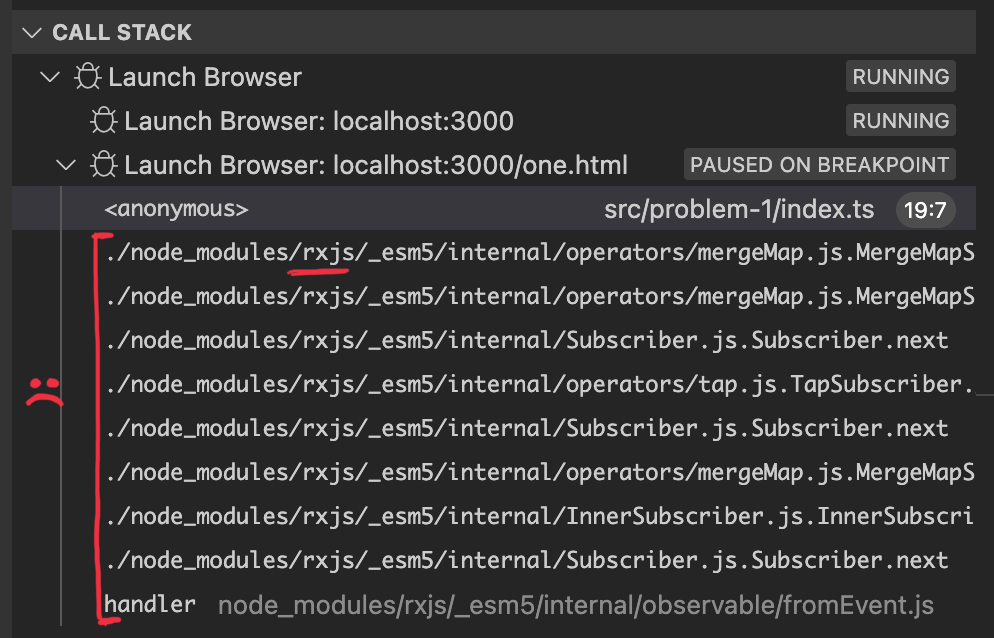
\includegraphics[height=\textheight/2]{figures/stacktrace.png}
        \caption{Stack Trace}
    \end{figure}
\end{frame}

\note[itemize] {
    \item Often felt lost though
    \item Stack traces
    \item program step controls: Operator? No: Internals!
    \item What else is possible?
}

\begin{frame}[fragile]{Debugging: The Reality}
    \begin{figure}[H]
        \centering
        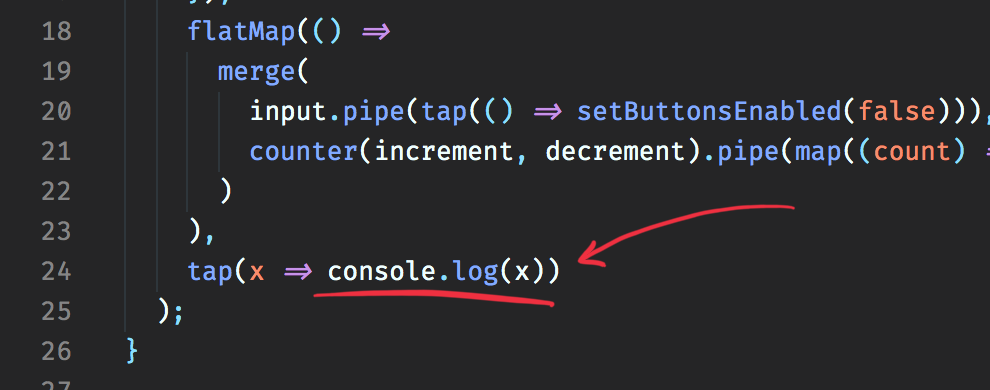
\includegraphics[height=\textheight/2]{figures/consolelog.png}
        \caption{Add Trace Logs}
    \end{figure}
\end{frame}

\note[itemize] {
    \item Especially when stuff gets complicated
    \item Debugging === Trace Logs
    \item Sprinkle log statements
}

\begin{frame}[fragile]{Debugging: The Reality}
    \begin{figure}[H]
        \centering
        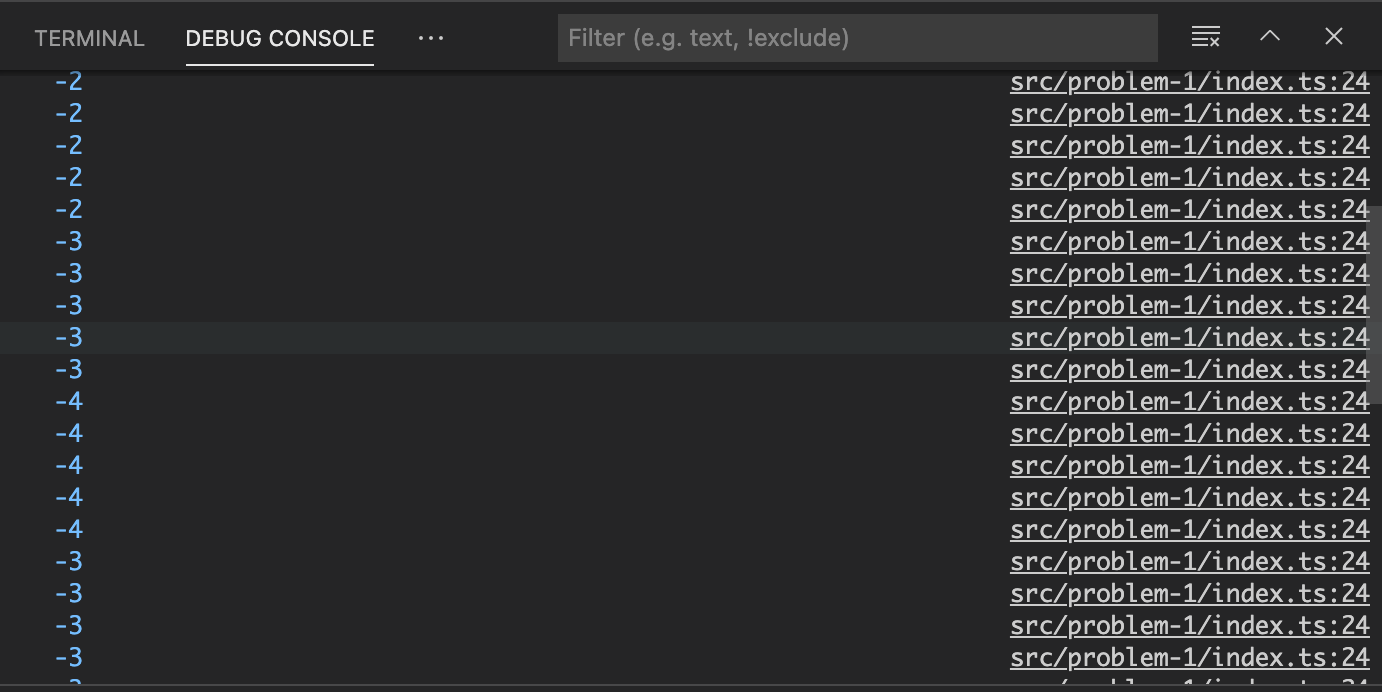
\includegraphics[height=\textheight/2]{figures/tracelogs.png}
        \caption{Flood of Trace Logs}
    \end{figure}
\end{frame}

\note[itemize] {
    \item Analyze flood of logs
    \item Find problem
    \item Remove log states
    \item DONT remove the bug fix ;)
    \item This left me...
}

\begin{frame}[fragile]{Really?}
    \begin{figure}[H]
        \centering
        
\includegraphics[height=\textheight/2]{figures/person-shrugging_1f937.png}
        \caption{\tiny{Source: \url{https://emojipedia.org/person-shrugging/}}}
    \end{figure}
\end{frame}

\note[itemize] {
    \item Frustrated!
    \item Mature Software Engineer has to feel different
    \item Looked for existing solutions
}

\begin{frame}[fragile]{A New Hope?}
    \begin{vfilleditems}
        \item \textbf{Reactive Inspector} for REScala \cite{10.1145/2577080.2577083}, Salvaneschi et al. \cite{10.1145/2884781.2884815} \cite{10.1145/2889160.2893174}
        \item \textbf{RxFiddle}, Banken et al. \cite{10.1145/3180155.3180156}
        \item Better trace logs using \textbf{rxjs-spy} \cite{rxjsspy}
    \end{vfilleditems}
\end{frame}

\note[itemize] {
    \item Own research
    \item Some interesting findings
    \item Most elaborate: Reactive Inspector
    \item Salvaneschi et al
    \item REScala, Scala
    \item Some, but not a lot for RxJS
    \item rxfiddle, banken et al -> Visualizer Externally
    \item rxjs-spy: Better logs, but still: trace log approach
    \item MEH!
    \item Lets do this on our own!
    \item -> Started with research questions
}


\subsection{Research Questions}

\begin{frame}[fragile]{Research Questions}
    \begin{enumerate}
        \vfill\item[RQ1] \textbf{What challenges} do software engineers face when debugging RxJS-based applications?
        \vfill\item[RQ2] How can the \textbf{experience} of software engineers during the debugging process of RxJS-based applications \textbf{be improved}?
    \end{enumerate}
\end{frame}

\note[itemize] {
    \item Before we can improve, if at all
    \item We need data on what we should improve
    \item Thats question 1
    \item Based on this
    \item Propose a concept to make dev experience better
    \item Thats question 2
    \item Lets get started!
}


\section{Studies}

\begin{frame}[fragile]{Road Map}
    \begin{vfilleditems}
        \item Two qualitative studies
        \begin{enumerate}
            \vfill\item Preparatory study using \textbf{interviews} and \textbf{``war story'' reports}
            \vfill\item \textbf{Controlled experiment} to validate previously identified findings
        \end{enumerate}
    \end{vfilleditems}
\end{frame}

\note[itemize] {
    \item Worked with 14 software engineering professionals
    \item Conducted interviews
    \item Collected written reports
    \item Then validated this with controlled experiment
}

\subsection{Study 1: Interviews and War Stories}

\begin{frame}[plain, noframenumbering]{Study 1: Preparation}
  \centering
  \vfill
  {\fontsize{30}{40}\selectfont\color{white}{Interviews\\and War Stories}}
  \vfill
\end{frame}

\begin{frame}[fragile]{Call for Participants}
    \begin{figure}[H]
        \centering
        
\includegraphics[height=0.6\textheight]{figures/tweet-interview.png}
        \caption{\tiny{Source: \url{https://twitter.com/swissmanu/status/1242429409208029185}}}
    \end{figure}
\end{frame}

\note[itemize] {
    \item Recruiting via Twitter and Email
    \item 10 participants
    \item Daily users of RP
    \item One RxJS Core team member
    \item Two Google Dev Experts on Angular
}

\begin{frame}[fragile]{Scope}
    \begin{columns}[T]
        \begin{column}{.4\linewidth}
            \begin{itemize}
                \item Five \textbf{Interviews}\vspace{1em}
                \begin{itemize}
                    \item General \textbf{Experience} with Reactive Programming\vspace{0.7em}
                    \item What do you \textbf{like}?\vspace{0.7em}
                    \item What do you \textbf{dislike}?
                \end{itemize}
        	\end{itemize}
        \end{column}
        \begin{column}{.4\linewidth}
            \begin{itemize}
                \item Five War Story \textbf{Reports}\vspace{1em}
                \begin{itemize}
            		\item Recall a specific \textbf{challenging} debugging situation?\vspace{0.7em}
            		\item How did you \textbf{solve} it?
        		\end{itemize}
        	\end{itemize}
        \end{column}
    \end{columns}
\end{frame}

\note[itemize] {
    \item Experience with RP
    \item Pros
    \item Cons / Pain Points
    \item They should recall particular scenario
    \item Step by step
    \item What problems?
    \item How did they solve them?
}

\begin{frame}[fragile]{Mentioned Debugging Techniques}
    \begin{figure}
        \centering
        \begin{tikzpicture}
            \pie[
                cloud,
                sum=10,
                after number={\textvisiblespace times},
                text=inside,
                radius=3,
                rotate=100,
                color={pureminimalistic@text@red}
            ]{
                3/Debugger,
                5/Trace Logs,
                2/Add. Tool
            }
        \end{tikzpicture}
    \end{figure}
\end{frame}


\note[itemize] {
    \item Repeating themes
    \item Debugging is hard
    \item Unsatisfying traditional debuggers
    \item Most often manual trace logs
    \item Or code extraction to to external tools
}

{
\setbeamercolor{background canvas}{bg=pureminimalistic@text@white}
\setbeamercolor{frametitle}{bg=pureminimalistic@text@white}
\setbeamercolor{normal text}{fg=pureminimalistic@text@black}
\begin{frame}[fragile, plain]{Key Take Aways}
    \begin{figure}
        \centering
        
\includegraphics[width=.7\textheight]{figures/rxjs-red-reveal-pattern.png}
        \caption{\tiny{Source: Manuel Alabor}}
    \end{figure}
\end{frame}

\note[itemize] {
    \item What do we get from this?
    \item Engineers use manual code modification
    \item Either trace logs
    \item Or extraction to external tools
    \item But why?
    \item Because traditional tools fail them
    \item These tools cant see through RxJS abstractions
}

\begin{frame}[fragile, plain]{Key Take Aways}
    \begin{figure}
        \centering
        
\includegraphics[width=.7\textheight]{figures/rxjs-red-reveal-pattern-lens.png}
        \caption{\tiny{Source: Manuel Alabor}}
    \end{figure}
\end{frame}

\note[itemize] {
    \item Hence, if given the correct filter
    \item In other words, a tool that sees through RxJS
    \item They could debug with less manual intervention
    \item Improve efficiency
    \item Improve quality because no code changes
    \item If manual code modification is really common practice...
}
}


\section{Study 2: Observational Study}

\begin{frame}[plain, noframenumbering]{Study 2: Observational Study}
    \centering
    \vfill
    {\fontsize{30}{40}\selectfont\color{white}{Controlled Experiment}}
    \vfill
\end{frame}


\note[itemize] {
    \item Is something we had to validate
    \item In a Controlled Experiment
    \item Obviously, we created hypothesis after previous findings...
}

\subsection{Study Design}

\begin{frame}[fragile]{Hypothesis}
    \begin{vfilleditems}
        \item[\Large{``}] If software engineers must solve an RxJS-based problem, then they \textbf{will instrument the code manually} in order to understand its behavior.
    \end{vfilleditems}
\end{frame}

\note[itemize] {
    \item Open to all manual modifications
    \item trace logs
    \item extracts
}

\begin{frame}{Study Design}
    \begin{vfilleditems}
        \item \textbf{Observational Study}
        \item \textbf{Briefing} upfront for every subject
        \item \textbf{Uncontrolled} Environment
        \item \textbf{Remote} moderation and execution
        \item ``After Action'' \textbf{Survey}
    \end{vfilleditems}
\end{frame}

\note[itemize] {
    \item Remotely conducted observational study
    \item Execution on subjects computer
    \item Individual dev environment
    \item Mimic "Daily dev routine"
    \item Two problems, 25 minutes each
    \item ~1h total
    \item Unattended survey afterwards -> RxJS experience data
}

\begin{frame}{Problem 1: Example}
    \begin{columns}[b]
        \begin{column}{.5\linewidth}
            \begin{figure}
                \centering
                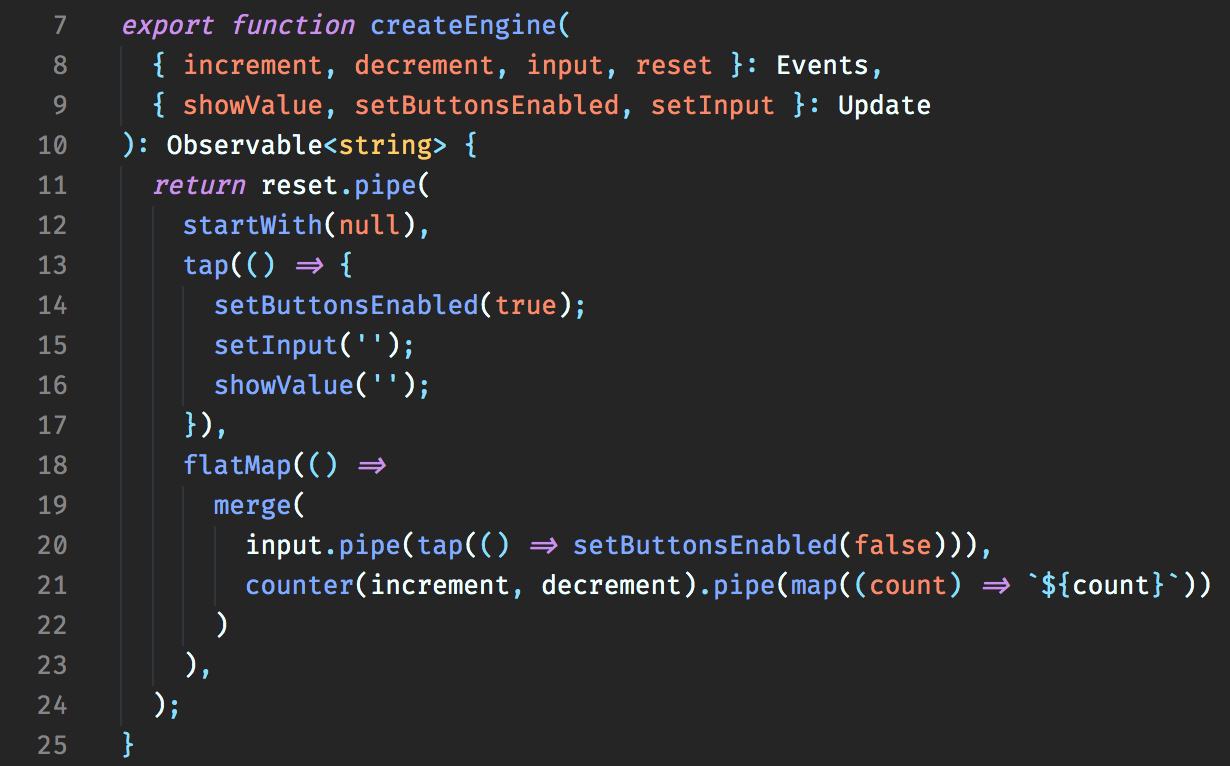
\includegraphics[width=.9\linewidth]{figures/problem1-code.png}
                \caption{RxJS Observable}
            \end{figure}
        \end{column}
        \begin{column}{.5\linewidth}
            \begin{figure}
                \centering
                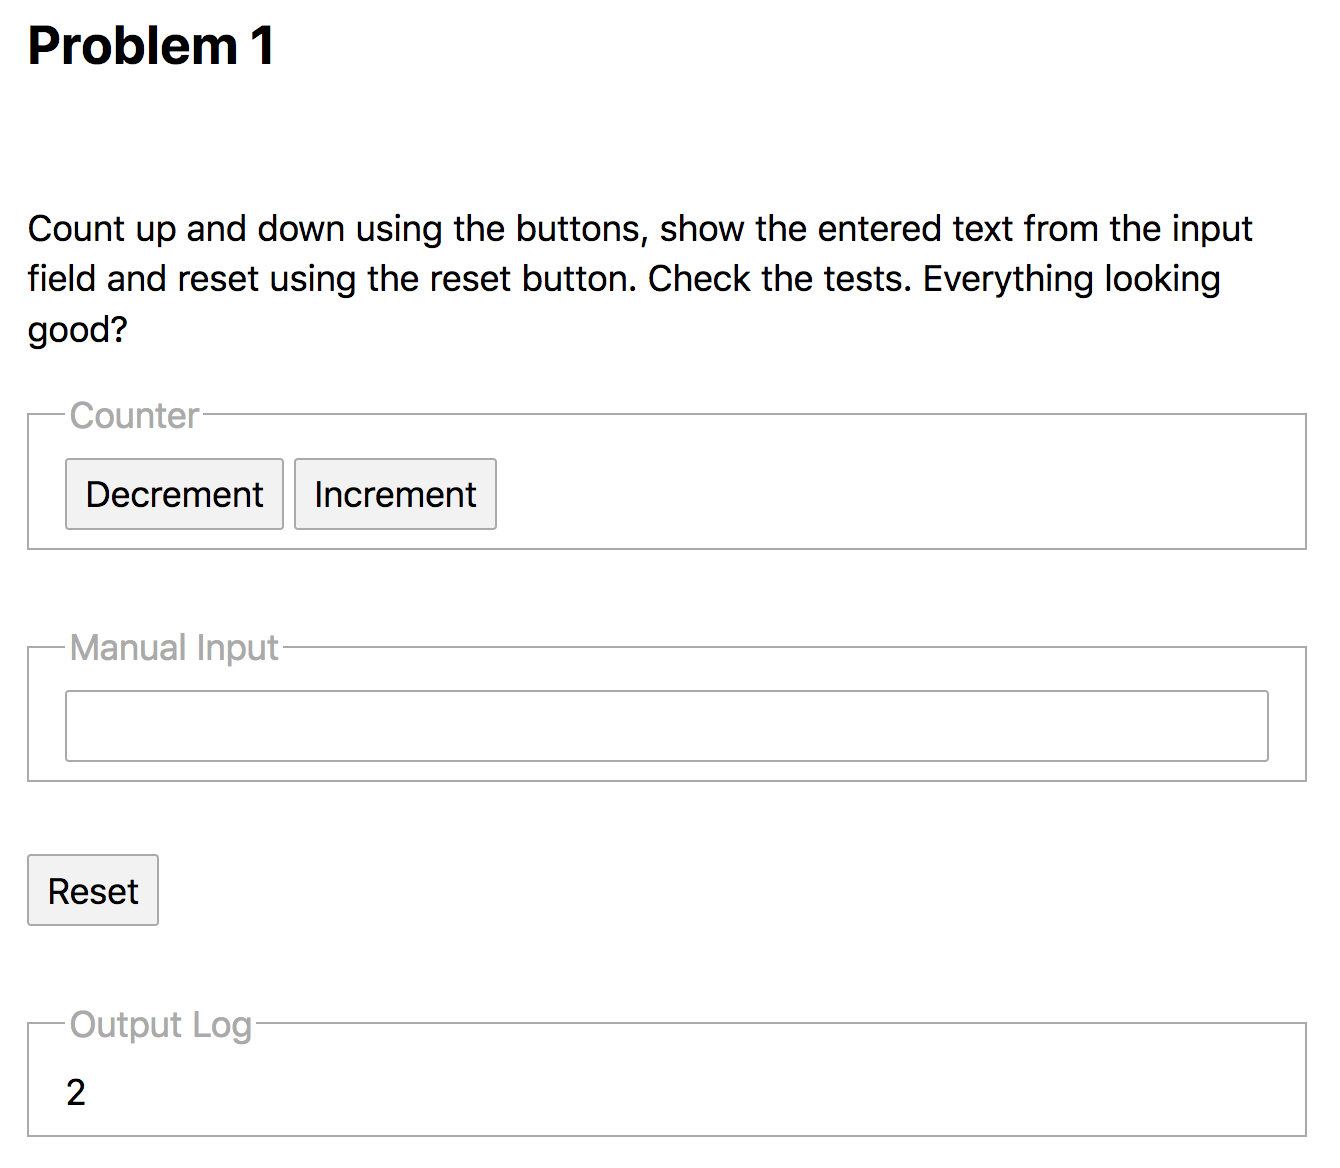
\includegraphics[width=.9\linewidth]{figures/problem1-ui.png}
                \caption{User Interface}
            \end{figure}
        \end{column}
    \end{columns}
\end{frame}

\note[itemize] {
    \item A problem consisted of:
    \item TypeScript \textbf{Code}, \textbf{Unit Tests}, runnable \textbf{UI}
    \item Goal: "We want to know how you debug!"
    \item Task: Identify and Resolve Bugs
    \item Task: "Speak out loud"
}

\subsection{Study Execution}

\begin{frame}{Subject Population}
    \begin{vfilleditems}
        \item \textbf{Four} professional software engineers
        \item Two currently \textbf{work} with RxJS
        \item Three have \textbf{two or more years} of \textbf{experience} with RxJS
        \item One of them uses RxJS to develop \textbf{backend applications}
    \end{vfilleditems}
\end{frame}

\note[itemize] {
    \item Four engineers recruited from personal network
    \item Experienced population; most >2y
    \item All use RxJS for frontend development
    \item One also for backend
}

\subsection{Study Results}

\begin{frame}[fragile]{Typically Used vs. Observed Uses}
    \begin{figure}
        \centering
        \begin{tikzpicture}
            \begin{axis}[
                    height=0.6\textheight,
                    width=0.8\linewidth,
                    xbar,
                    xtick={0,1,2,3,4},
                    symbolic y coords={Add. Tools,Debugger,Trace Logs},
                    ytick=data,
                    enlarge y limits=0.5,
                    enlargelimits=0.15,
                    nodes near coords, nodes near coords align={horizontal},
                    legend pos=south east,
                    legend style={fill=none,at={(0.5,-0.2)},anchor=north},
                    legend cell align={left},
                    reverse legend
                ]
                
                \addlegendentry{\# of subjects were observed using}
                \addplot[
                        fill=pureminimalistic@text@red,
                        draw=pureminimalistic@text@red
                    ]
                    coordinates {
                        (0,Add. Tools) (4,Trace Logs) (2,Debugger)
                    };
                
                \addlegendentry{\# of subjects typically use}
                \addplot[
                        pattern=crosshatch dots,
                        pattern color=pureminimalistic@text@red,
                        draw=pureminimalistic@text@red
                    ]
                    coordinates {
                        (2,Add. Tools) (4,Trace Logs) (3,Debugger)
                    };
            \end{axis}
        \end{tikzpicture}
    \end{figure}
\end{frame}

\note[itemize] {
    \item Based on survey and experiment
    \item Able to compare typically vs observed
    \item Trace logs: 100\% used and told to typically use
    \item Debugger: Some small difference, not all use typically
    \item Interpretation: Already gave up on debugger?
    \item Largest discrepancy: Add. tools!
    \item No one used them
    \item \textbf{Even though survey told they usually do!}
    \item Even if they had personal dev setup at home
    \item Therefore, we reason...
}

\section{Conclusion}

\begin{frame}[fragile]{Interpretation}
    \begin{vfilleditems}
        \item If Engineers \textbf{know} about RxJS debugging tools, they \textbf{do not use} them
        \item \textbf{Manual code modification} is common practice
        \item \textbf{Imperative} debuggers cannot handle RxJS abstractions
    \end{vfilleditems}
\end{frame}

\note[itemize] {
    \item Knowing about tools seems not enough
    \item Is there a \textbf{boundary} that keeps engineers from using them?
    \item Eventually, tendency to trace logs and code extraction
    \item Repeated theme: Traditional debuggers cannot help in all cases
    \item In summary, this builds basis for answer to RQ1
}

\begin{frame}[fragile]{Answer}
    \begin{enumerate}
        \item[\color{gray}{RQ1}] \color{gray}{What challenges do software engineers face when debugging RxJS-based applications?}
        \vfill\item[\Large{``}] \color{white}{The most significant challenge software engineers face [\dots] is to know \textbf{when} they should apply \textbf{what tool} to resolve their current problem in the \textbf{most efficient} way.}
    \end{enumerate}
\end{frame}

\note[itemize] {
    \item Challenge: What tool, when and how
    \item Often: The "next best" as we saw: Traditional tools
    \item Often: Modify code
    \item Less often: Specific tools
    \item What can we do about it?
    \item Answer question 2
}

\begin{frame}[fragile]{Answer}
    \begin{enumerate}
        \item[\color{gray}{RQ2}] \color{gray}{How can the experience of software engineers during the debugging process of RxJS-based applications be improved?}
        \vfill\item[\Large{``}] \color{white}{[\dots] \textbf{improve} the \textbf{experience} of debugging [\dots] by providing RP specific debugging utilities where software engineers expect them the most: \textbf{Fully integrated} [\dots into] their IDE [\dots]}
    \end{enumerate}
\end{frame}

\note[itemize] {
    \item Improve the dev user experience
    \item Lower the boundary to use the right tool
    \item At the right time
    \item Integrate the right tools where they are expected the most
    \item Dont look for it: Its there where it belongs.
    \item Hence, outlook to future work...
}

\section{Future Work}

\begin{frame}[fragile]{Future Work}
    \begin{vfilleditems}
        \item \textbf{Propose} and \textbf{implement} solution to \textbf{prevent} manual code \textbf{modification}
        \item \textbf{Evaluate} proposal on \textbdf{effectiveness} in follow up study
    \end{vfilleditems}
\end{frame}

\note[itemize] {
    \item Work on a concrete prototype
    \item Find solution for manual code modification scenarios
    \item Without manual intervention required
    \item Validate effectiveness in another study iteration
}

\begin{frame}[plain, noframenumbering]
  \centering
  \vfill
  {\fontsize{40}{50}\selectfont\color{white}{Q \& A}}
  \vfill
\end{frame}

\note[itemize] {
    \item Happy for input
    \item Happy to answer questions
}

\appendix
\begin{frame}[allowframebreaks]{References}
	\printbibliography
\end{frame}

\begin{frame}[plain, noframenumbering]{}
    \centering
    \vfill
    {\fontsize{30}{40}\selectfont\color{white}{Backup Slides}}
    \vfill
\end{frame}

\begin{frame}[fragile]{Future Work PoC: Add Probe}
    \begin{figure}[H]
        \centering
        \includegraphics[height=0.6\textheight]{figures/tweet-rxjs-debugging-extension.png}
        \caption{\tiny{Source: \url{https://twitter.com/swissmanu/status/1313412280072232960}}}
    \end{figure}
\end{frame}

\begin{frame}[fragile]{Future Work PoC: Monitor}
    \begin{figure}[H]
        \centering
        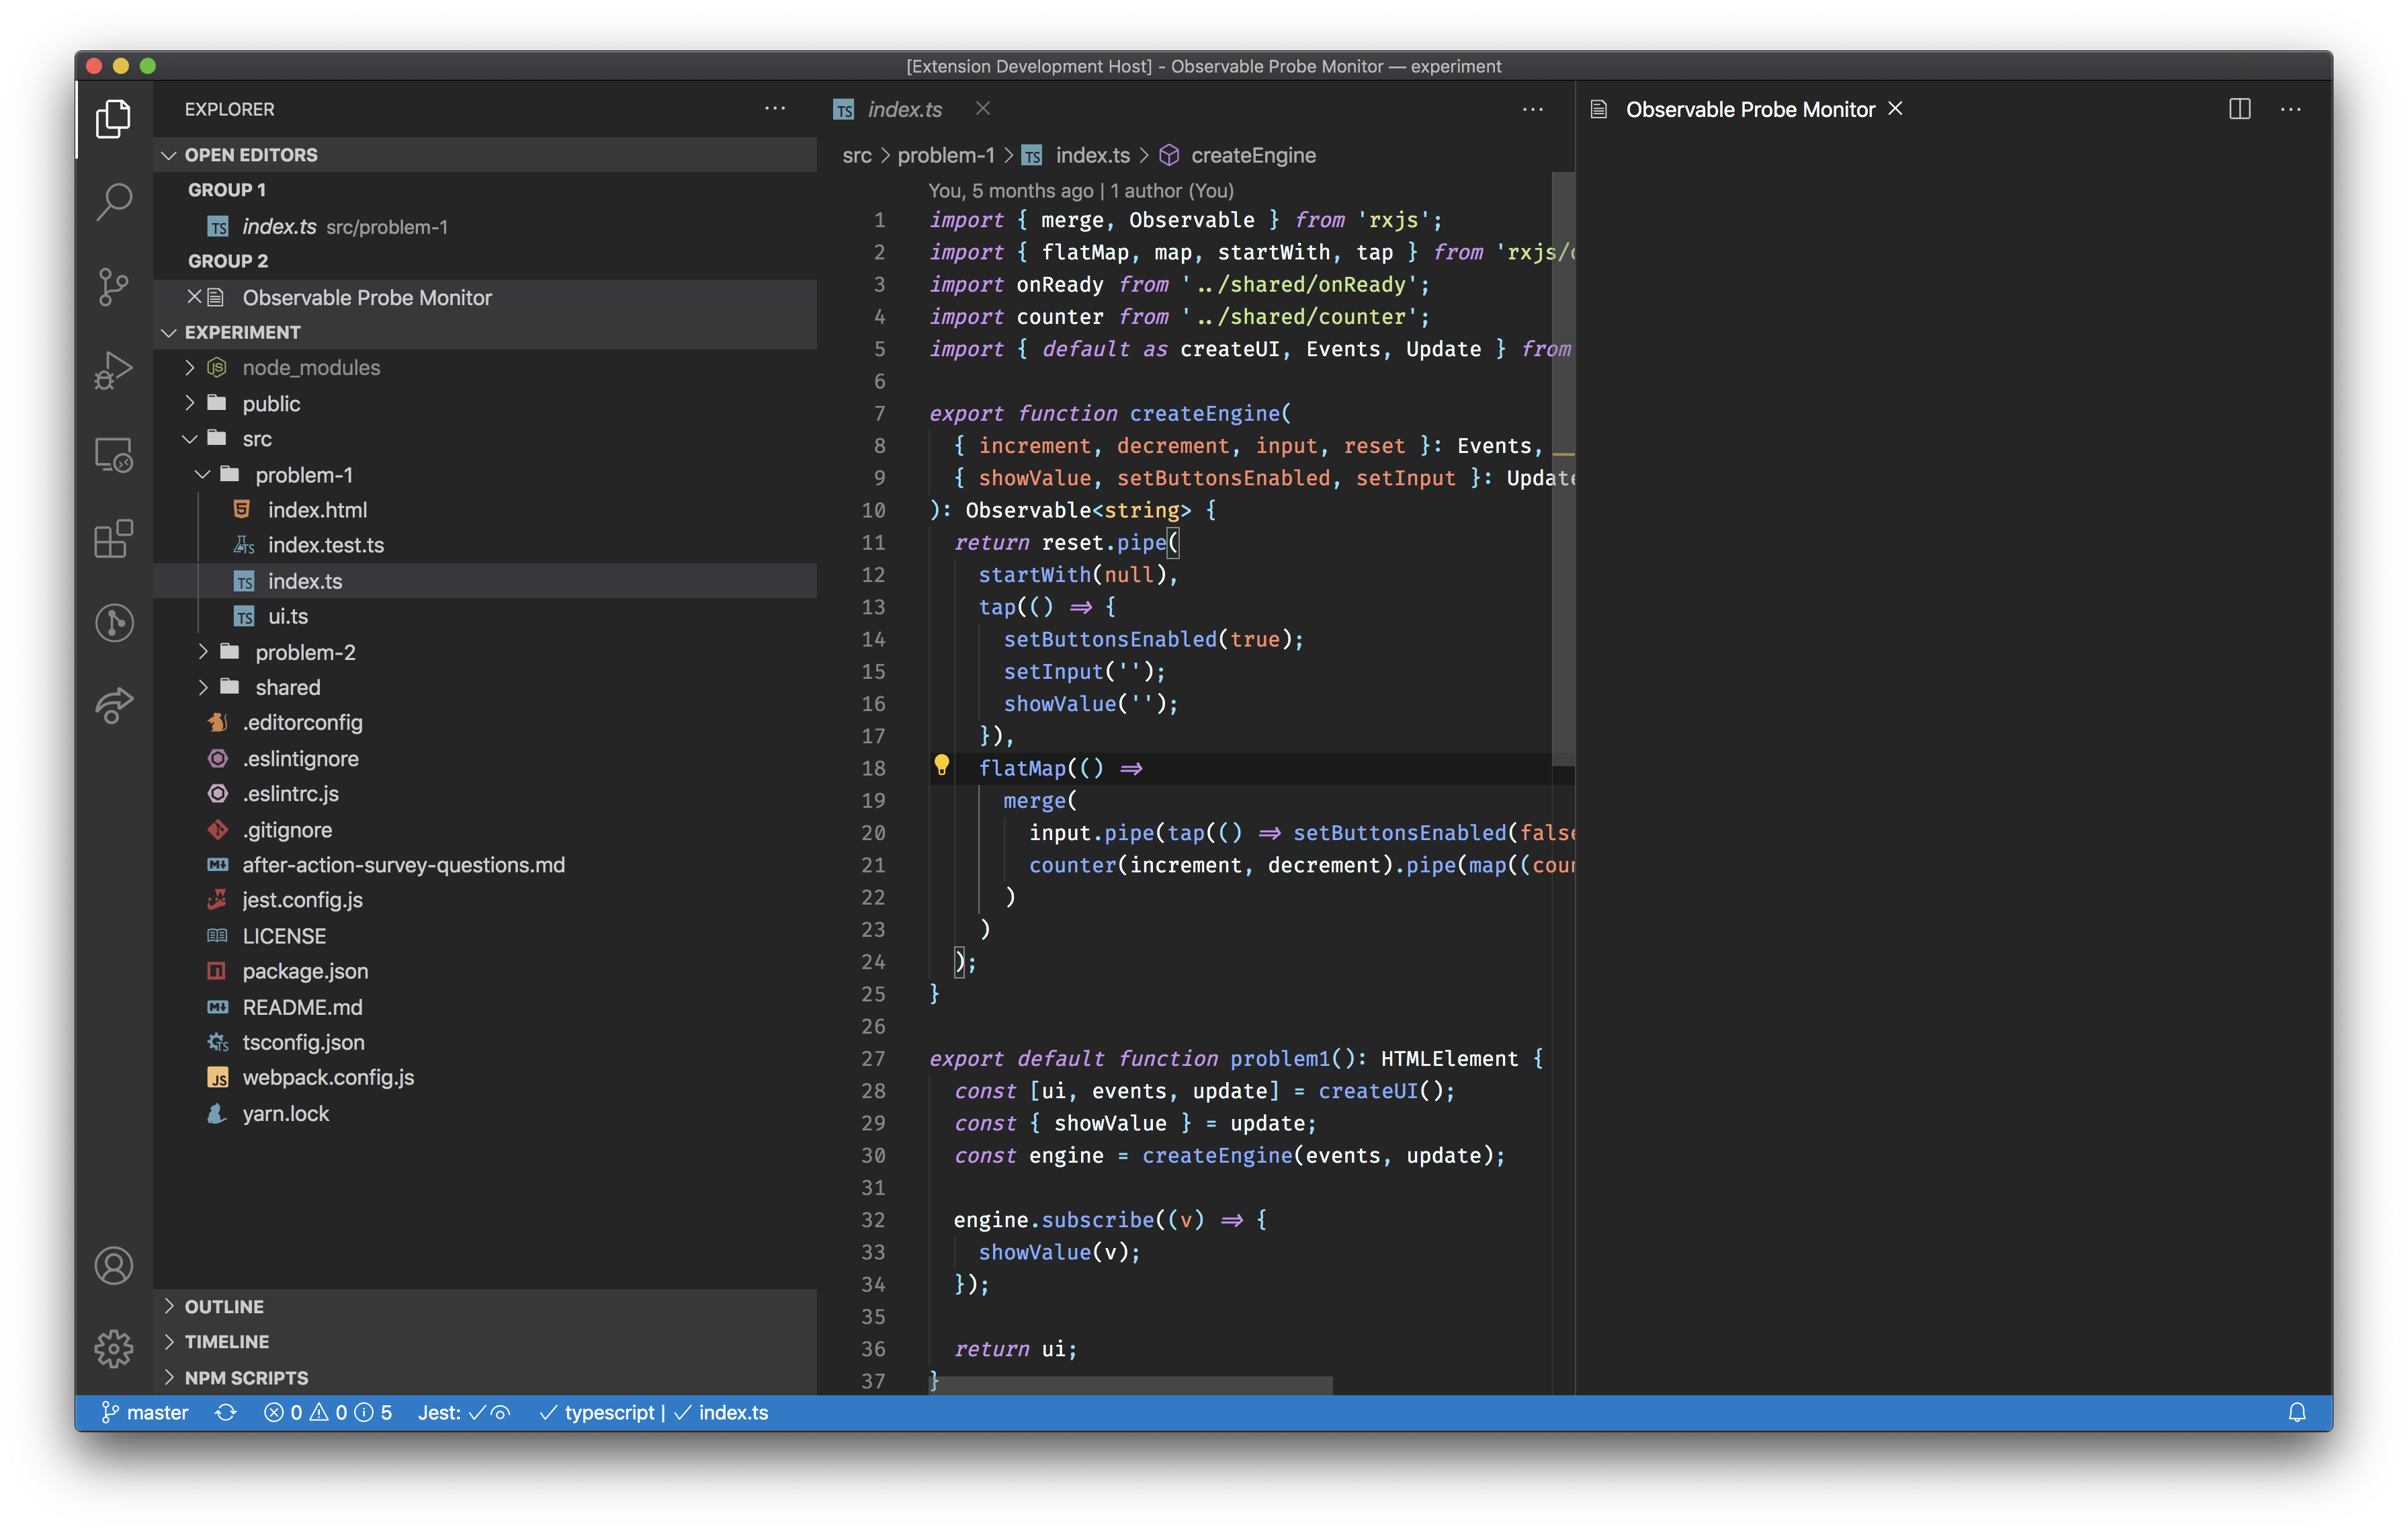
\includegraphics[height=0.7\textheight]{figures/backup-screenshots/step5-2.png}
        \caption{Empty Monitor Pane (right)}
    \end{figure}
\end{frame}

\begin{frame}[fragile]{Future Work PoC: Output}
    \begin{figure}[H]
        \centering
        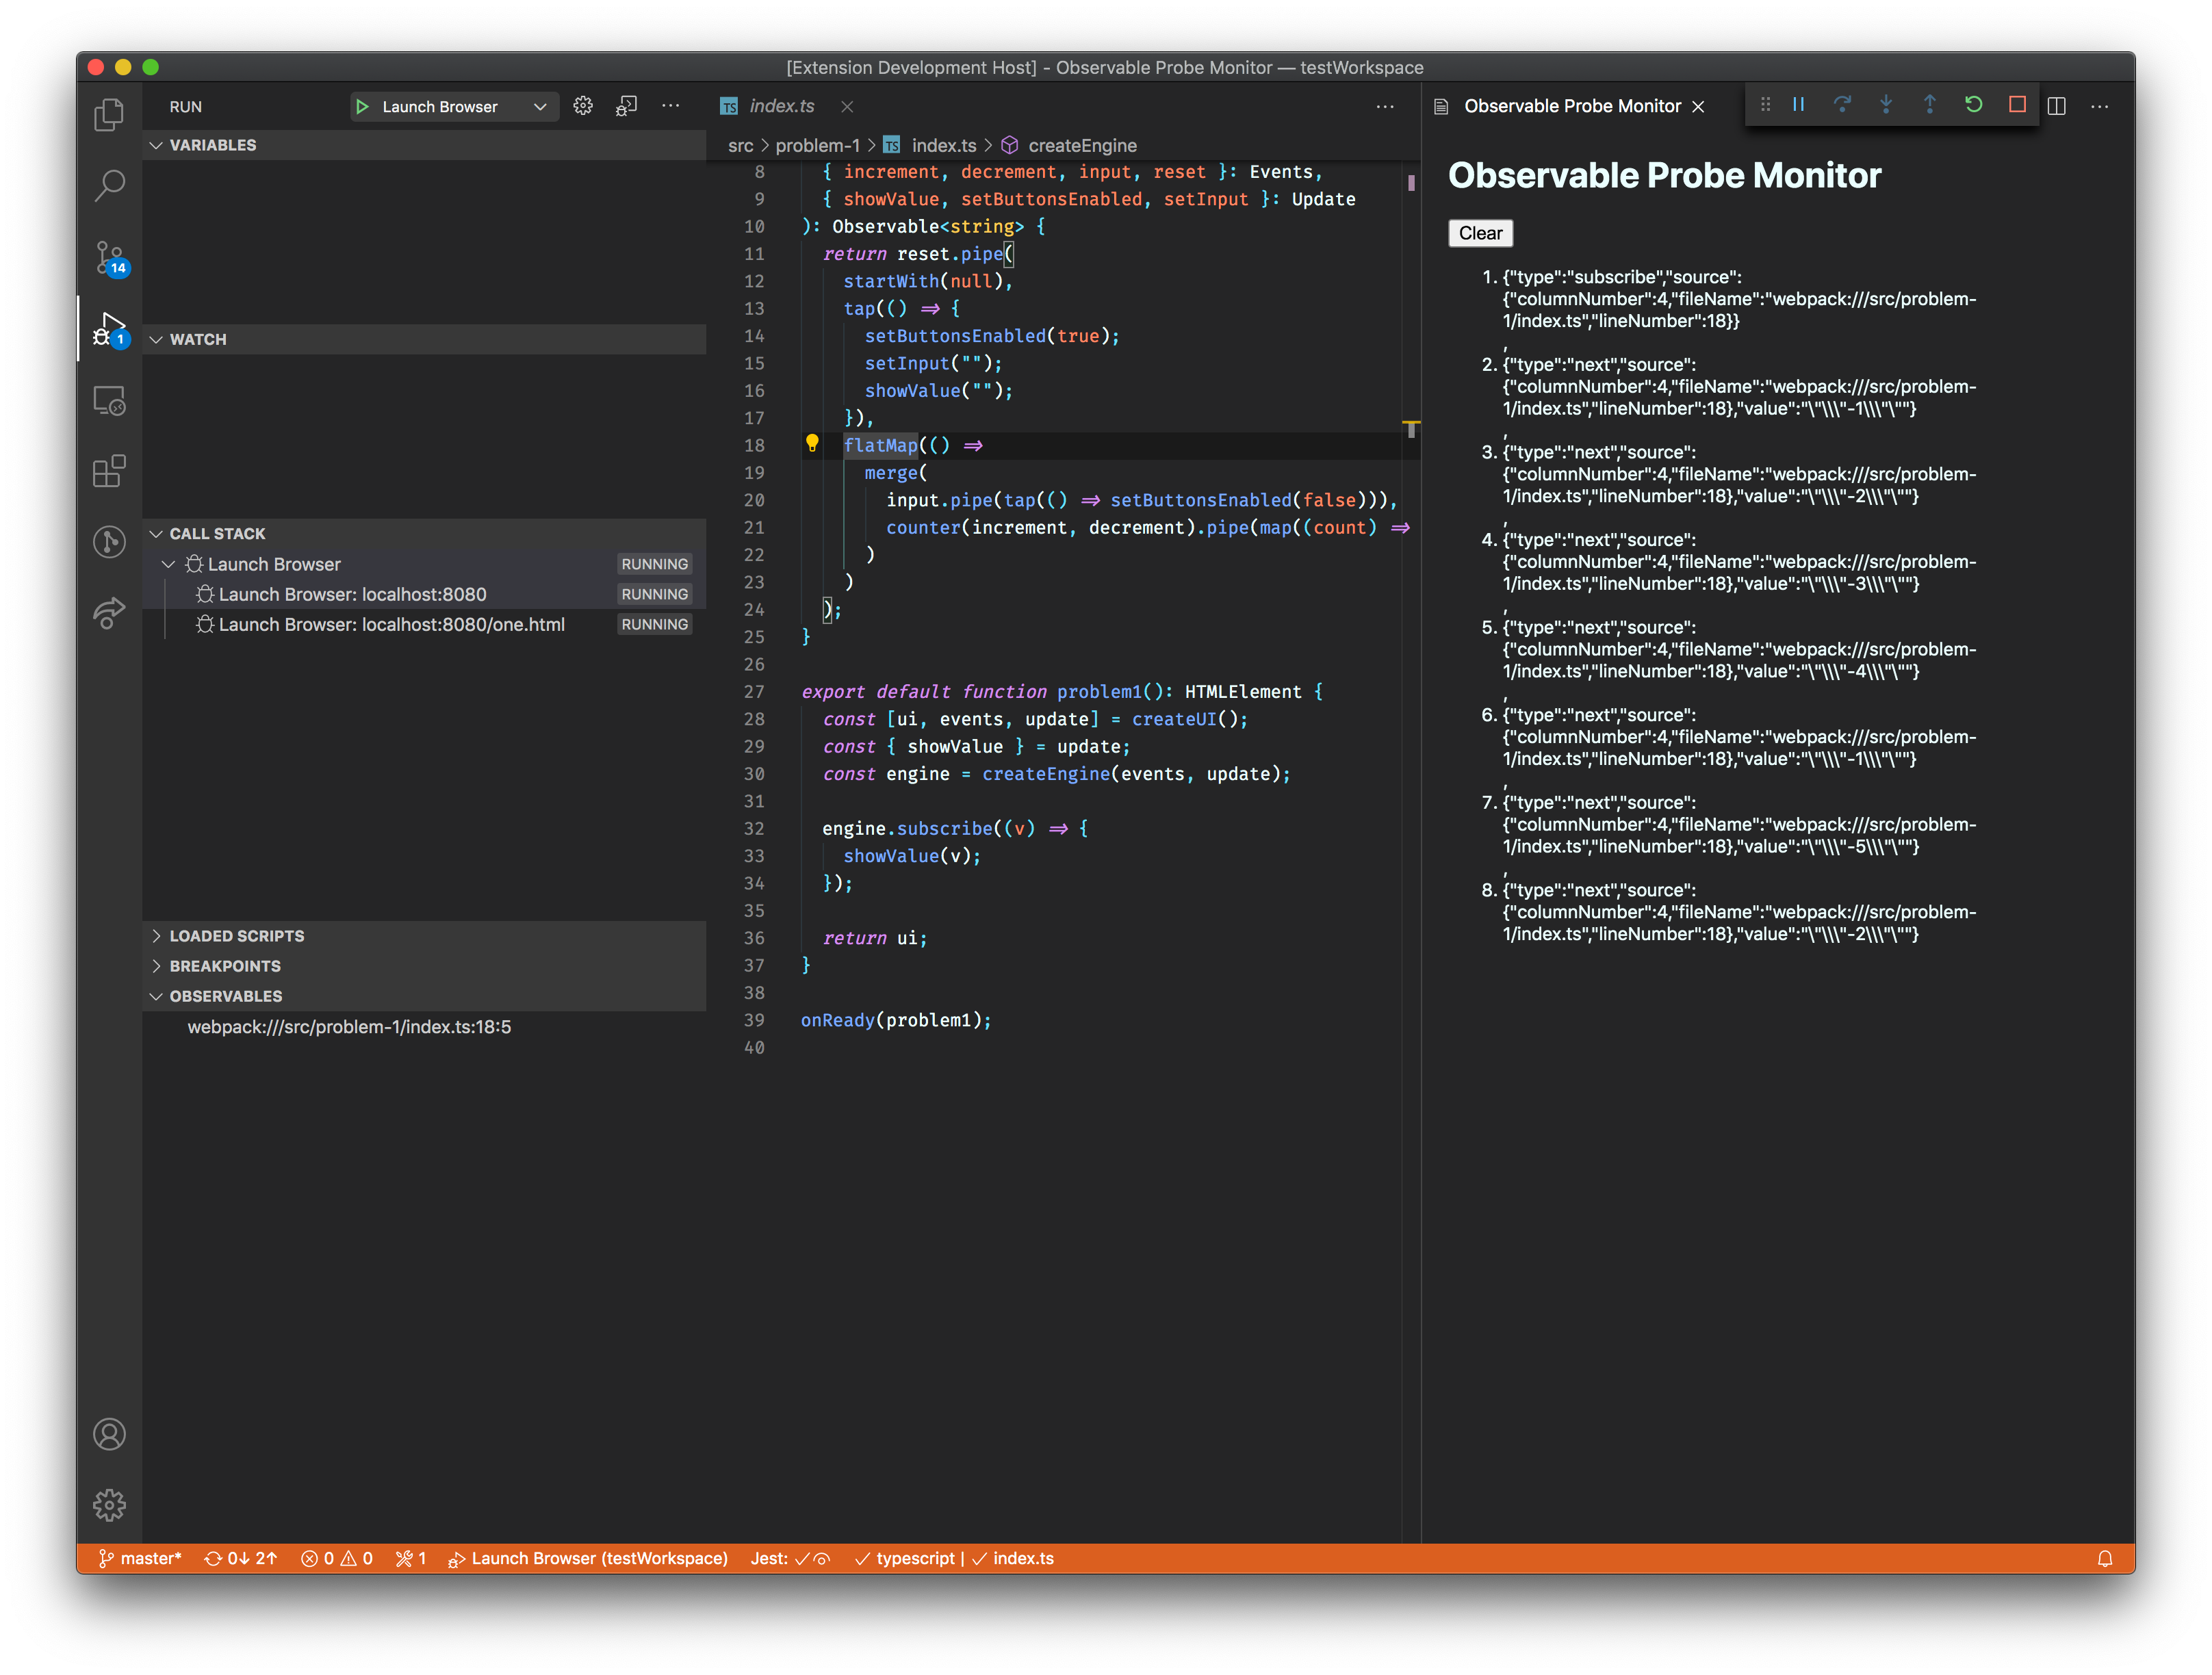
\includegraphics[height=0.7\textheight]{figures/backup-screenshots/step8.png}
        \caption{Monitor Pane with Output (right)}
    \end{figure}
\end{frame}


\end{document}